\subsection{Distanz-Messungen}
Der Sensor wurde auf einem Breadboard mit einem Arduino Uno verbunden und übertrug die Werte
vie USB-Kabel an den Seriellen Monitor der Arduino IDE. Um eine Mögliche Schieflage auf dem
Breadboard abzufedern wurden aus 200 Messungen der Durchschnitt berechnet von den Werten vor
der Verarbeitung subtrahiert. So liegt der Sensor mathematisch absolut flach auf. \\
Insgesamt wurden 10 Tests pro Formel gemacht, die Ergebnisse können Sie unten einsehen.\\

\begin{figure} [h]
\centering
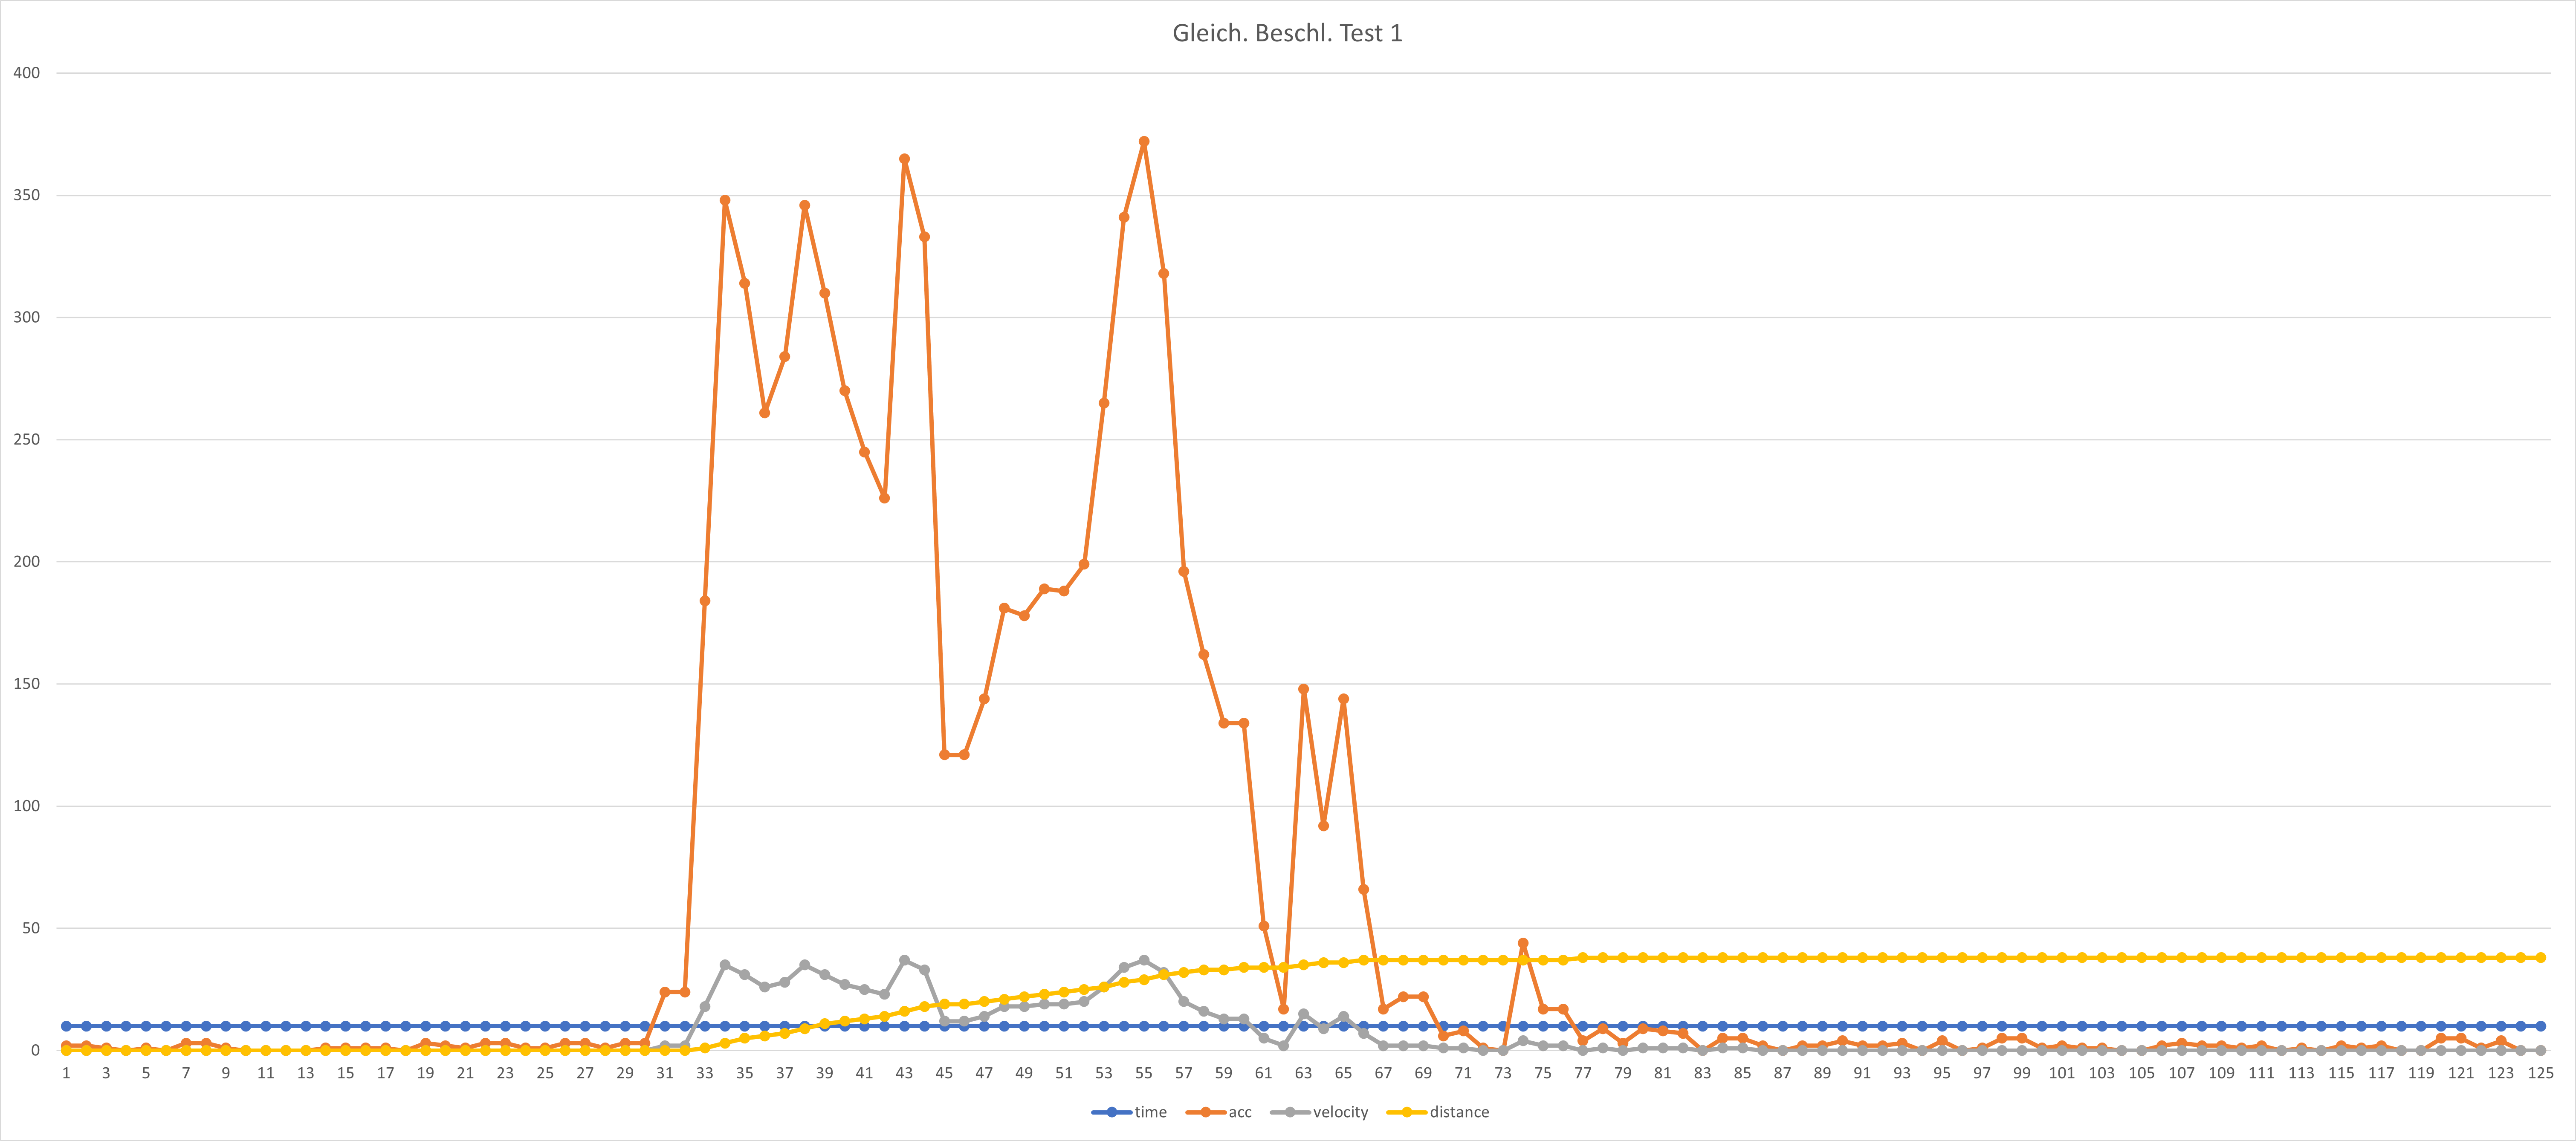
\includegraphics[width = 15cm]{Bilder/constDistance1}
\caption{Gleichmäßige Formel | Test 1}
%\label{fig:wo-bin-ich}
\end{figure}

\begin{figure} [h]
    \centering
    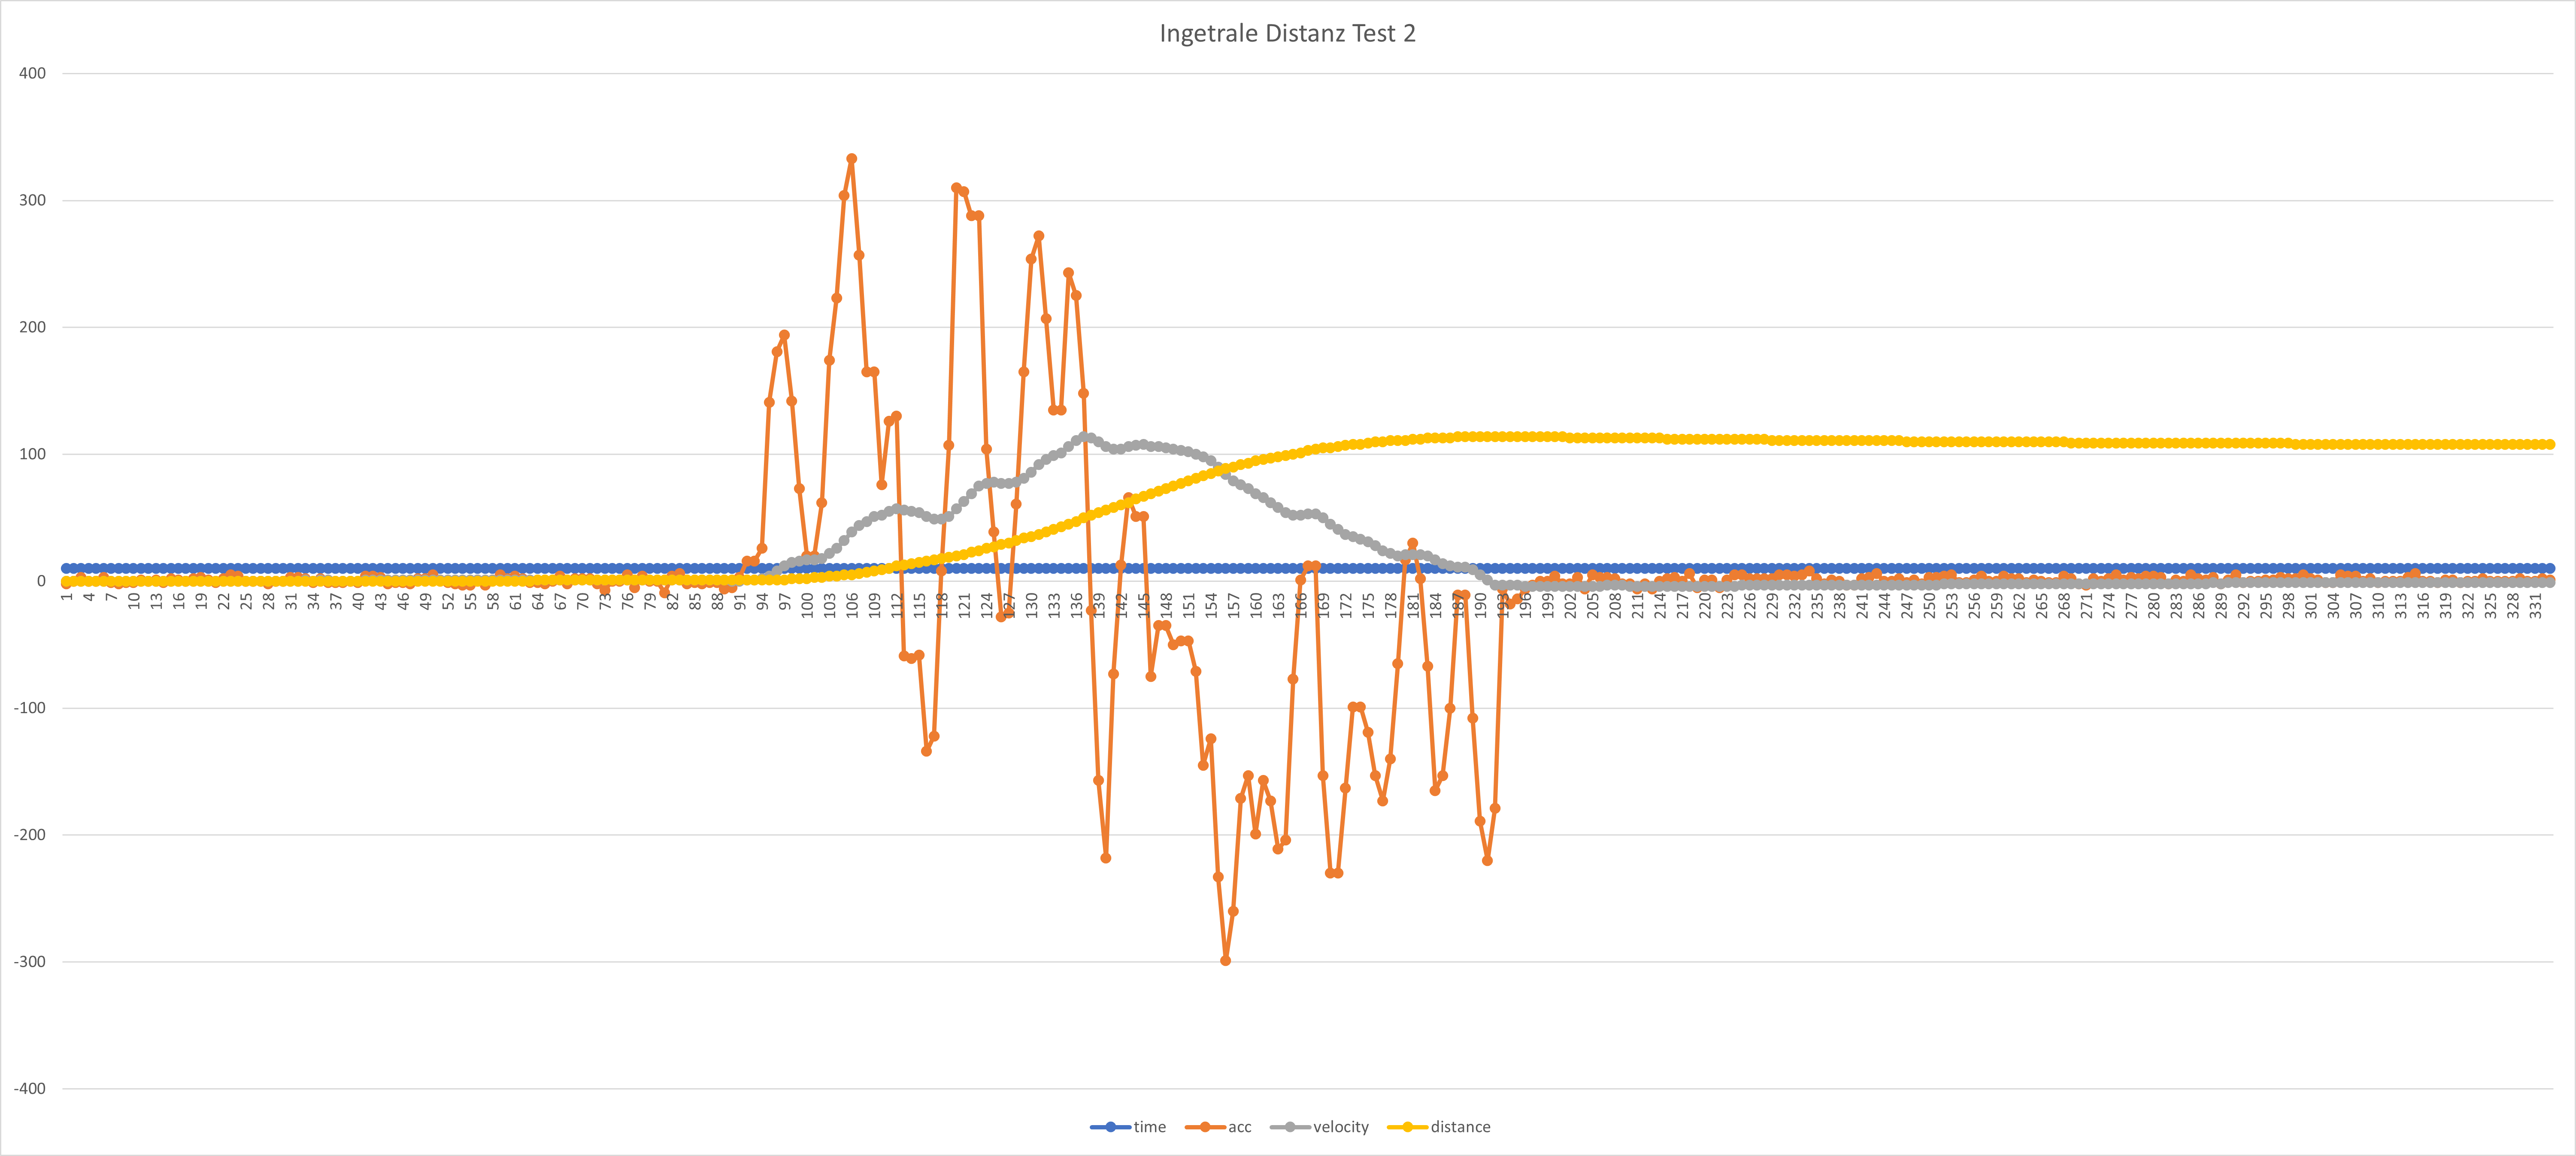
\includegraphics[width = 15cm]{Bilder/integralDistance2}
    \caption{Integrale Formel | Test 2}
    %\label{fig:wo-bin-ich}
    \end{figure}

\subsection{Fehler}
In den folgenden Graphen sind die Mess-Ergebnisse der Formeln veranschaulicht. Im ersten Graph
sind die Ergebnisse der 10 Distanz-Messungen miteinander verglichen. Der Sprung der
Ergebnisse bei der Integralen Formel ab Test 4 ist auf den Wechsel einen vermutlich fehlerhaften
Sensors zurück zu führen.\\
\\
Die zwei weiteren Graphen zeigen die Fehler bei 10 Sek"undigem Stillstand. Der exponentielle Drift 
bei der Integralen Formel ist typisch.


\begin{figure} [h]
    \centering
    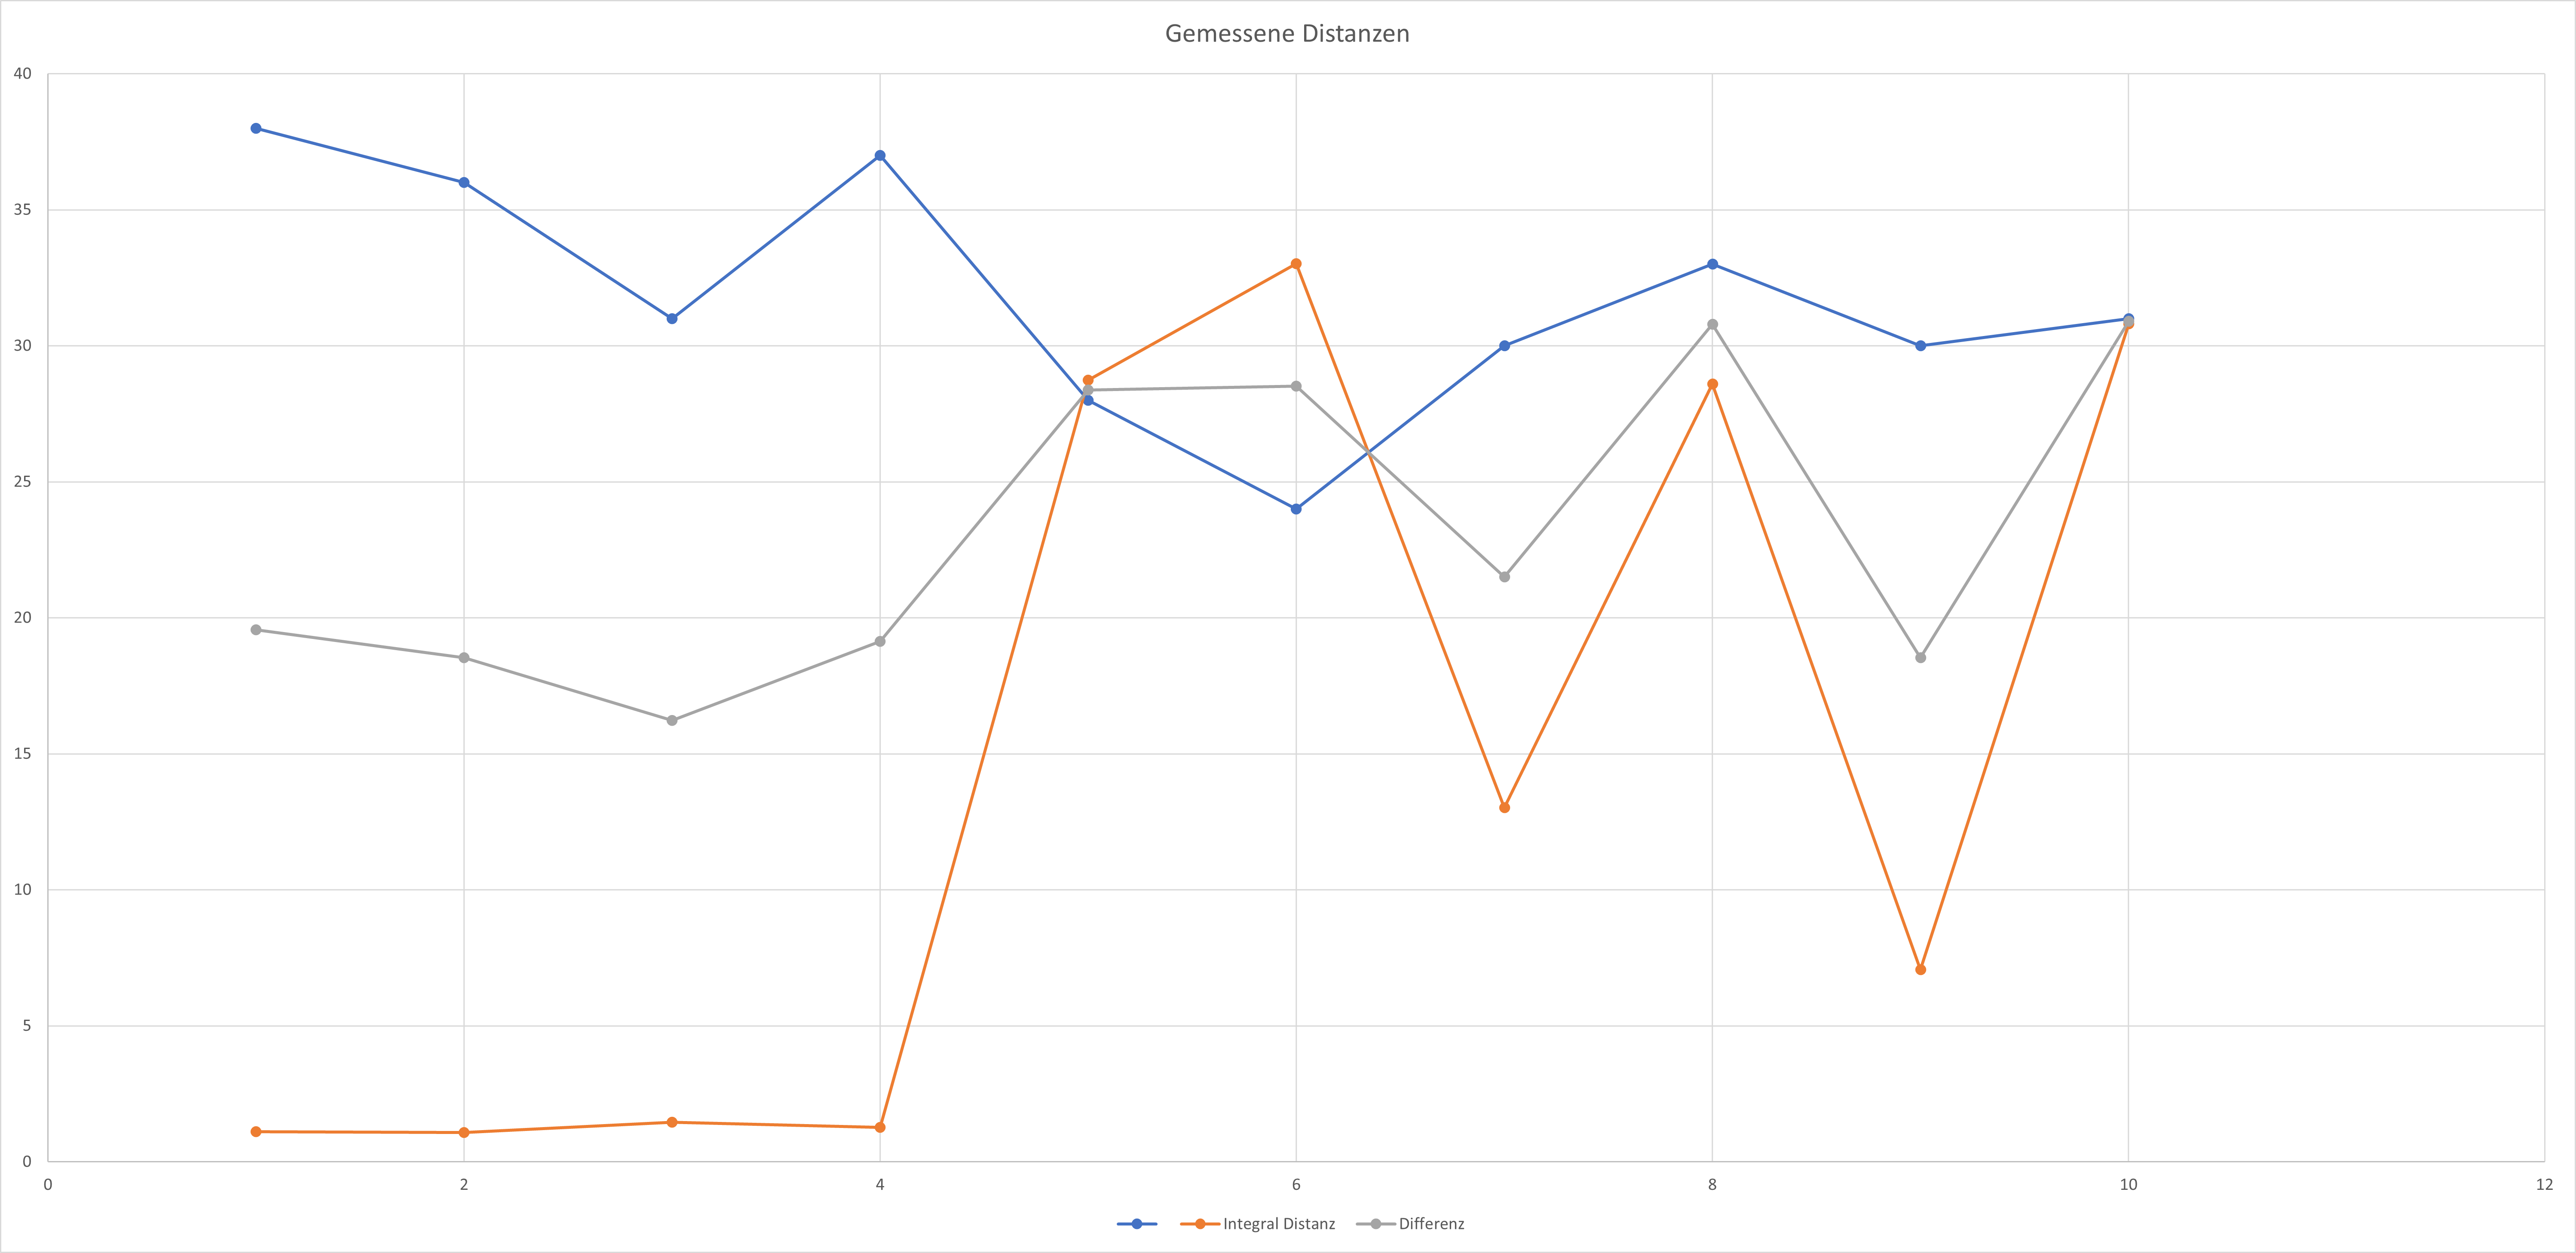
\includegraphics[width = 15cm]{Bilder/_DistanzVergleich}
    \caption{Integrale Formel | Test 2}
    %\label{fig:wo-bin-ich}
    \end{figure}


\begin{figure} [h]
    \centering
    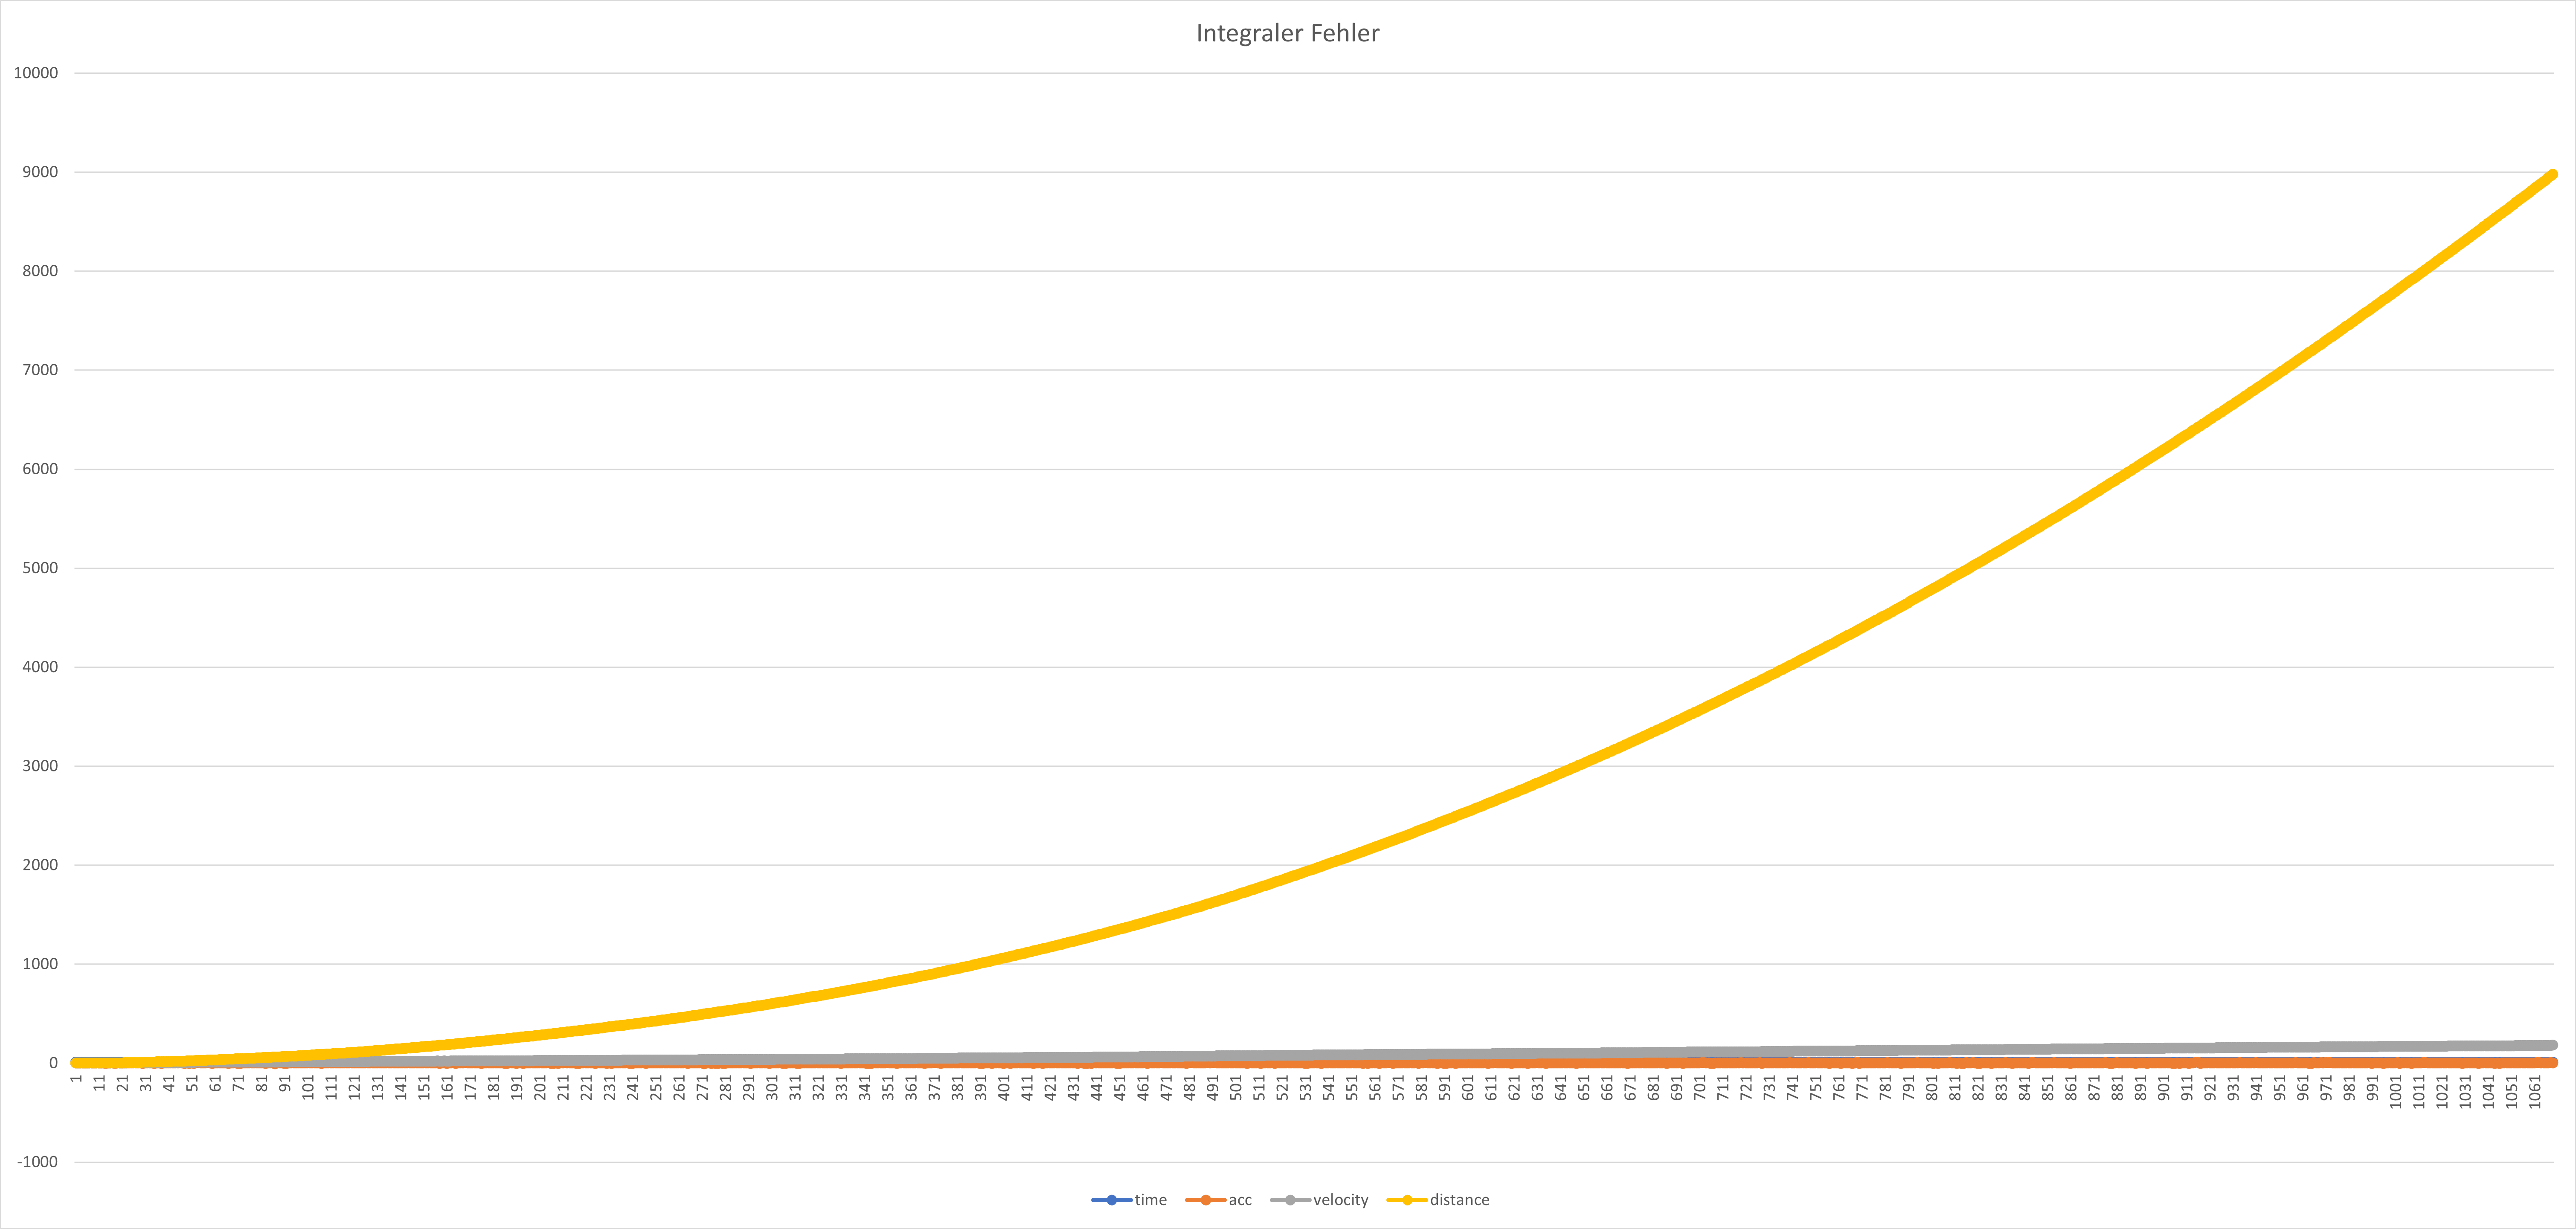
\includegraphics[width = 15cm]{Bilder/_integralDistance001}
    \caption{Integrale Formel | Test 2}
    %\label{fig:wo-bin-ich}
    \end{figure}

    \begin{figure} [h]
        \centering
        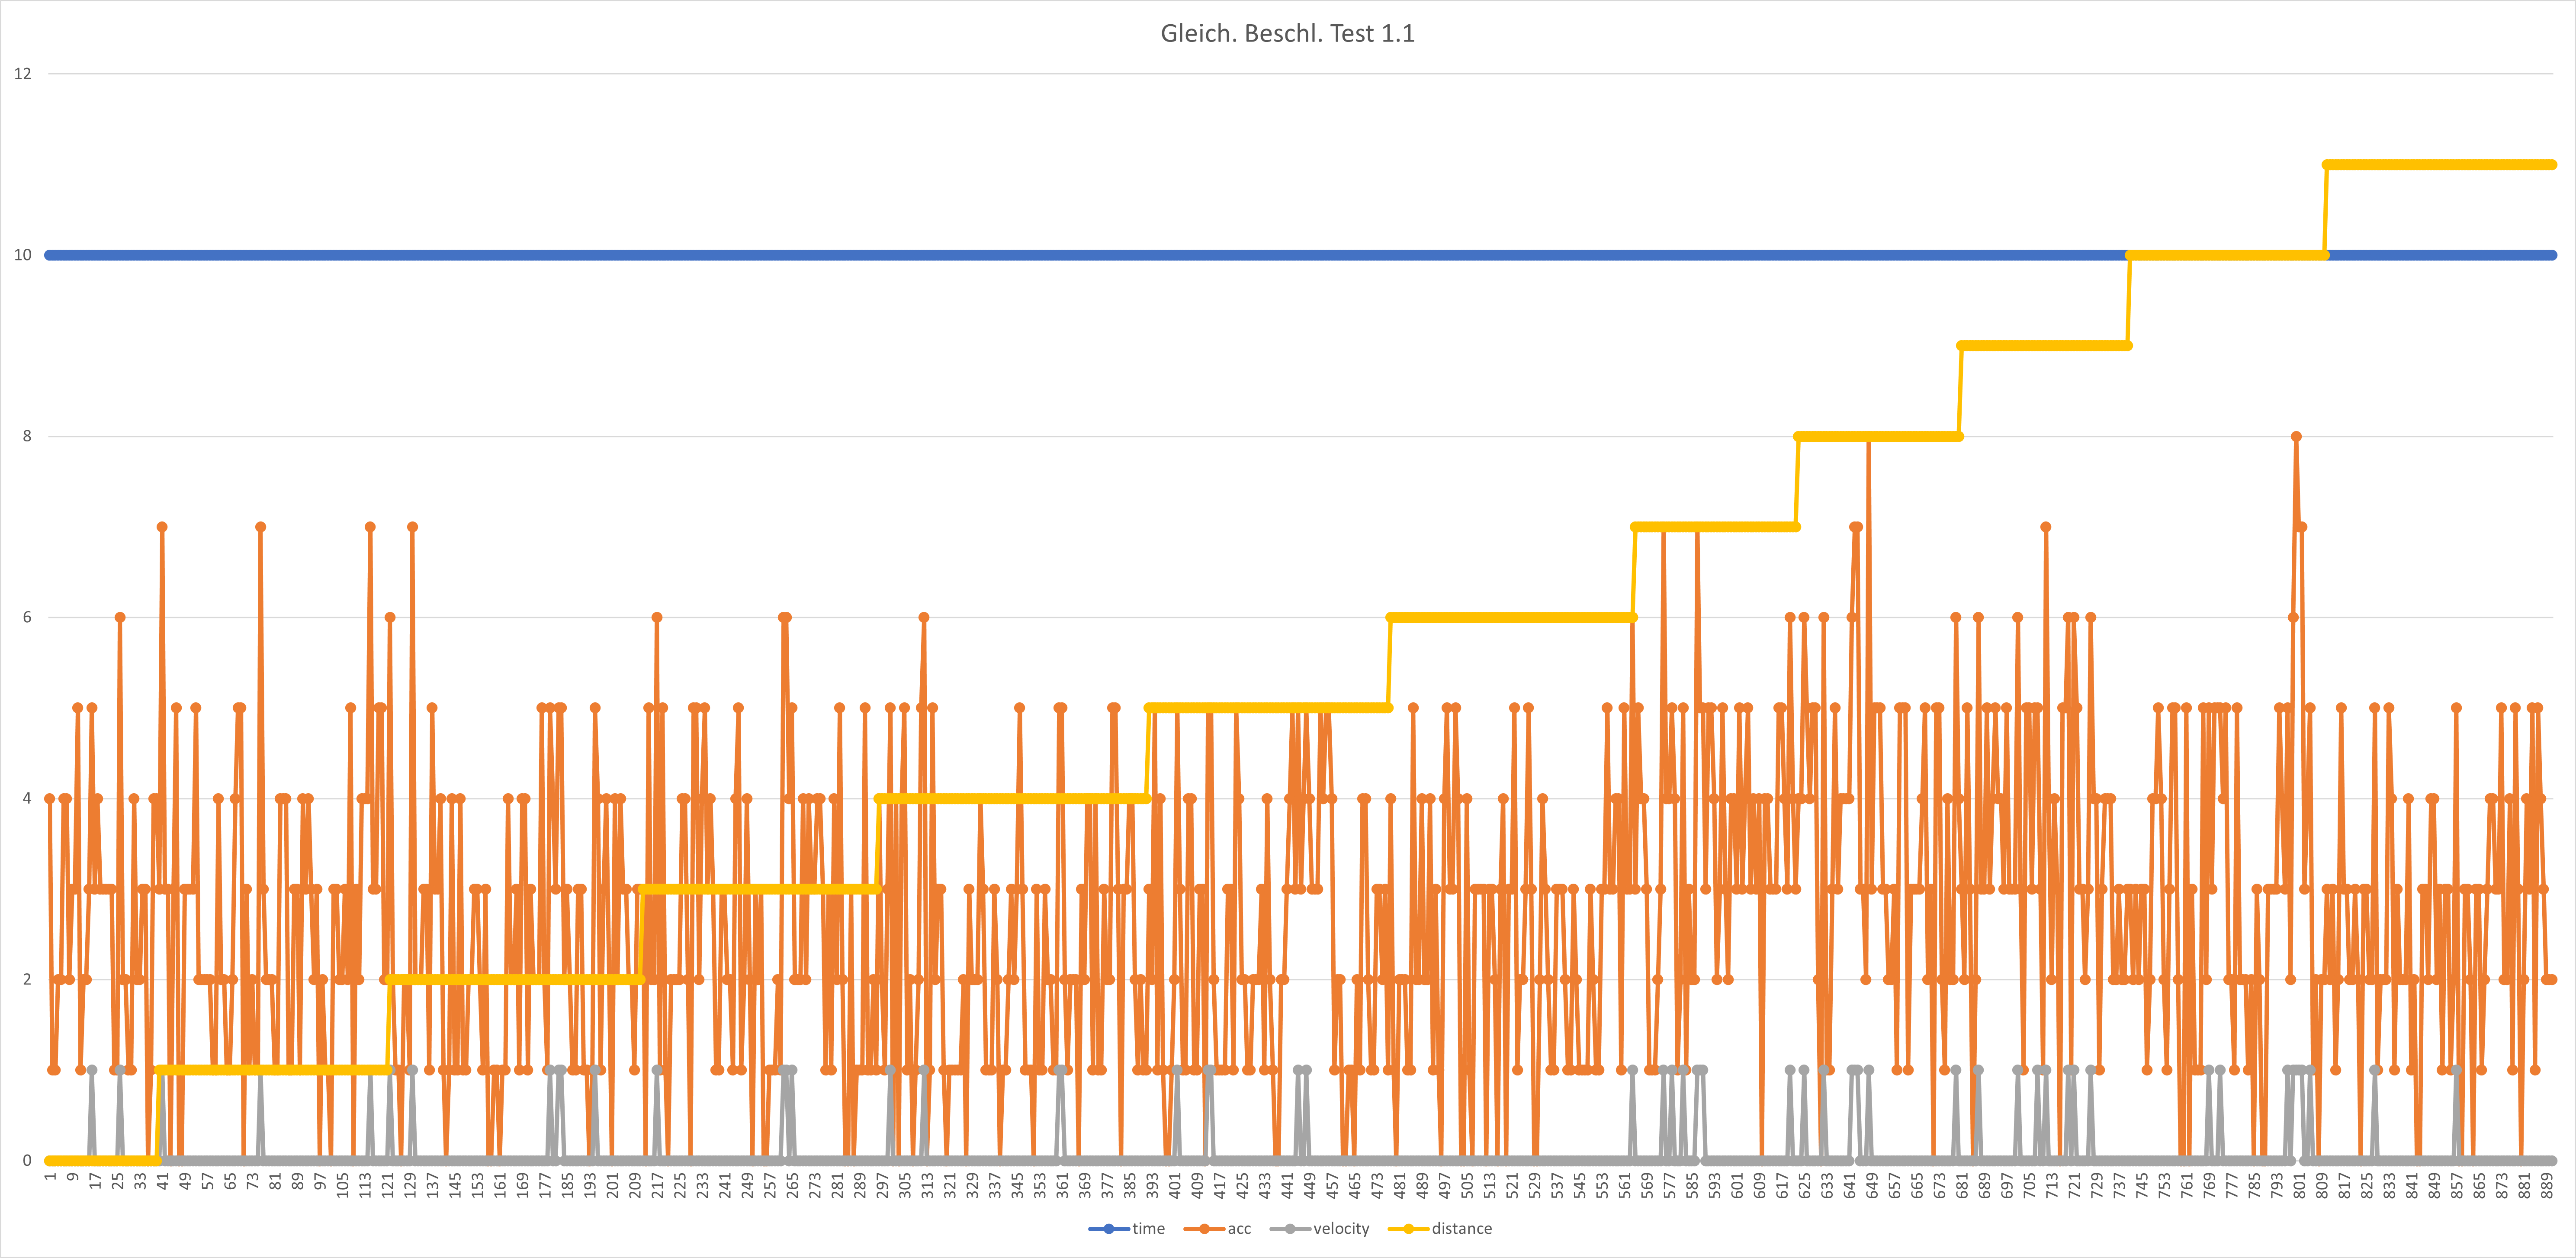
\includegraphics[width = 15cm]{Bilder/_constDistance001}
        \caption{Integrale Formel | Test 2}
        %\label{fig:wo-bin-ich}
        \end{figure}
    
